The classification scheme as described above has been used on the Banknote Authentication dataset \cite{banknote_paper} (downloaded from \cite{banknote_download}\footnote{Note that this page explains the labels the wrong way around. See \cite{genuine_class_banknote}}).
This particular dataset was chosen because it required only few particles to encode the input and the output:
\begin{enumerate}
	\item There are only two distinct labels (binary classification).
	\item Each input vector contains only four elements.
\end{enumerate}

The implementation is available at \url{https://github.com/Nifrec/nenwin} under the open-source AGPL-3.0 licence\cite{AGPL_3}.

\subsection{Task description}
The classification task is to classify banknotes as genuine or as forgeries, 
given four derived features from the images. 
Class 0 has 762 samples and represent the genuine banknotes,
class 1 has 610 represents the forgeries.
The derived features have been pre-computed, and are:
\begin{enumerate}
	\item Variance
	\item Skewness
	\item Kurtosis
	\item Entropy
\end{enumerate}

\subsection{Architectures}
Three different architectures have been designed and were evaluated. See also Fig. \ref{fig:banknote_architectures}.

\paragraph{Architecture A:}
\begin{itemize}
	\item Vertices of input region: (-2.5, -1), (-2.5, 1), (2.5, -1), (2.5, 1).
	\item 4 non-output nodes surrounding the input region (positions (0, -5), (-5, 0), (5, 0) and (0, 5)).
	\item MarbleEaterNodes (output Nodes) at (-10, 0) and (10, 0).
\end{itemize}

\paragraph{Architecture B:}
Same as Architecture A, but with additional Nodes at (2.5, 2.5), (-2.5, 2.5), (2.5, -2.5), (-2.5, -2.5).

\paragraph{Architecture C:}
\begin{itemize}
	\item Vertices of input region: (0, 0), (0, 1), (6, 0), (6, 1).
	\item 5 non-output nodes surrounding the input region (positions (1, 2), (2, 3), (3, 2), (4, 3) and (5, 2)).
	\item MarbleEaterNodes (output Nodes) at (1, 4) and (5, 4).
\end{itemize}

\begin{figure}
	\centering
	\begin{subfigure}[b]{0.3\textwidth}
		\centering
		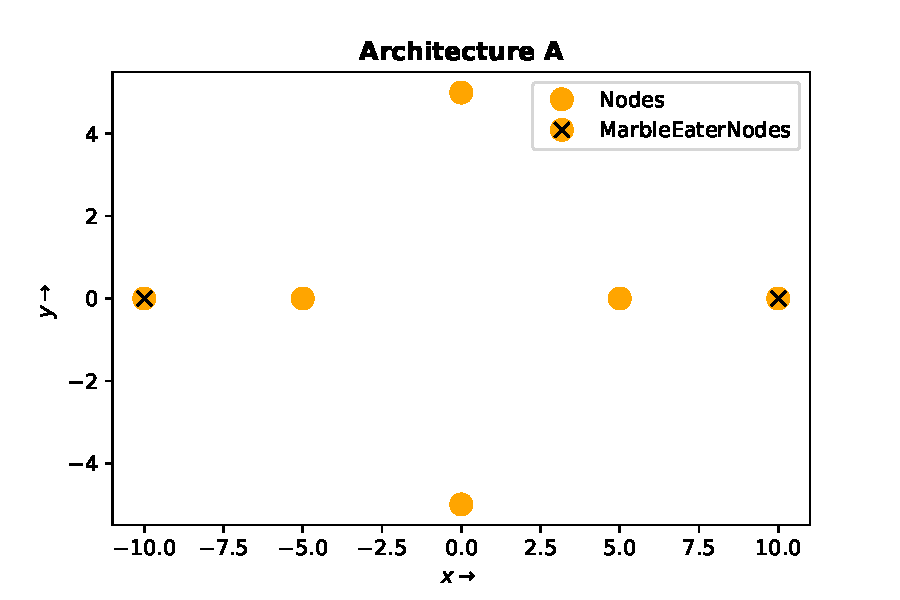
\includegraphics[width=\textwidth]{figures/architecture_A.pdf}
		\label{fig:architecture_a}
	\end{subfigure}
	\begin{subfigure}[b]{0.3\textwidth}
		\centering
		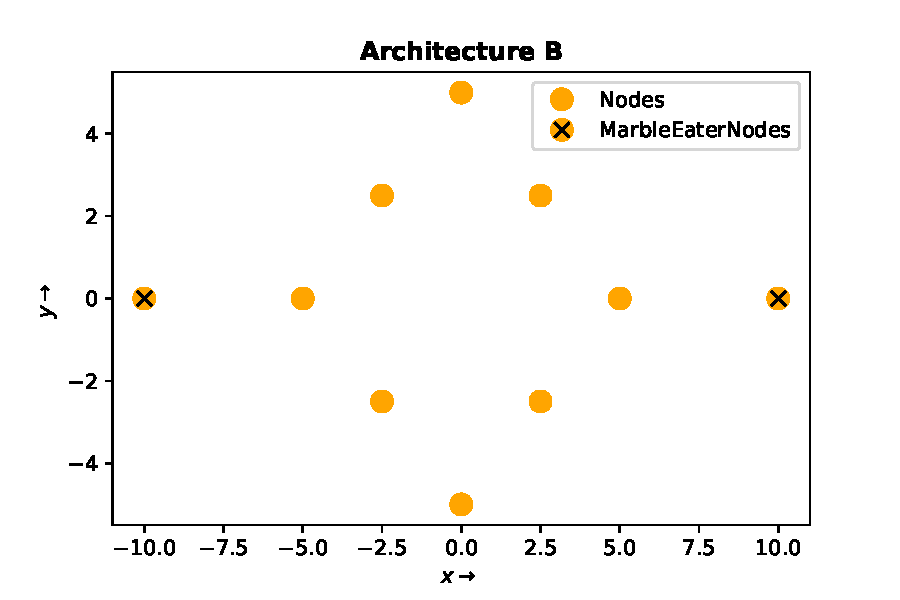
\includegraphics[width=\textwidth]{figures/architecture_B.pdf}
		\label{fig:architecture_b}
	\end{subfigure}
	\begin{subfigure}[b]{0.3\textwidth}
		\centering
		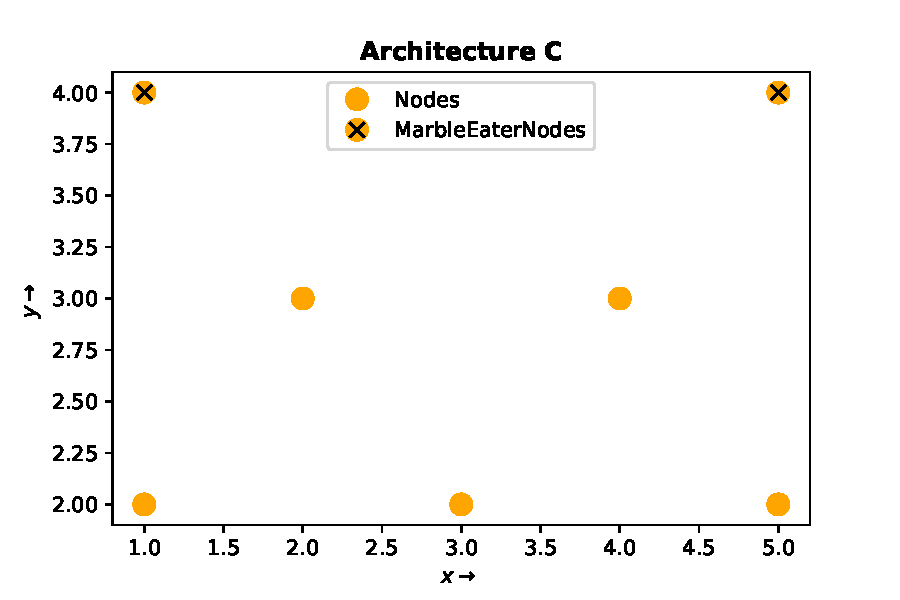
\includegraphics[width=\textwidth]{figures/architecture_C.pdf}
		\label{fig:architecture_c}
	\end{subfigure}

	\caption{\textsc{Nenwin} Architectures used for training on the banknote dataset.}
	\label{fig:banknote_architectures}
\end{figure}